\section{Anwendung}
\subsection{Projekt erstellen}
\subsubsection{Git-Repo initialisieren}

\subsubsection{Dateistruktur}
Abbildung \ref{fig:OrdnerDatei} zeigt die empfohlene Ordner und Dateistruktur für neue Projekte am Beispiel des "`HowTo"'-Projektes.
Die Ordner "`tikz"' und "`idiotenseite"' müssen natürlich nur erstellt werden wenn sie auch gebraucht werden. In allen Ordnernamen werden nur
Kleinbuchstaben verwendet, die einzige Ausnahme bildet der Hauptordner, welcher gleich benannt wird wie das offizielle Modulkürzel des Faches.
Die Hauptdatei (das ist diejenige in der \verb+\begin{document}+ \ldots \verb+\end{document}+ steht) wird ebenfalls nach dem Modulkürzel benannt.
Die einzelnen Kapitel (\verb+\section{}+) werden im Ordner \verb+sections+ abgelegt und nachher mit \verb+\input{}+ in das Hauptdokument eingebunden.
Der Dateiname sollte möglichst dem Titel des Kapitels entsprechen. Bilder und Grafiken welche mit externen Programmen erstellt wurden sind im Ordner
\verb+images+ abzulegen. Alles was zur Konfiguration des Layouts dient findet den Platz im \verb+header+ Ordner, TikZ-Grafiken werden im entsprechenden
\verb+tikz+ Ordner abgelegt.

\begin{figure}[h]
\centering
  \begin{tikzpicture}[%
	grow via three points={one child at (0.5, -0.8) and
	two children at(0.5,-0.8) and (0.5, -1.6)},
	edge from parent path={(\tikzparentnode.south) |- (\tikzchildnode.west)}]
	\tikzstyle{every node}=[anchor=west, minimum width=2.5cm, minimum height=0.6cm]
	\tikzstyle{folder}=[draw=black, thick]
	\tikzstyle{optional}=[dashed, folder]
	\node[folder] {HowTo}
		child {node[folder] {header}}
		child {node[folder] {sections}}
		child {node[folder] {images}}
		child {node[optional] {tikz}}
		child {node[optional] {idiotenseite}}
		child {node {HowTo.tex}};
  \end{tikzpicture}
  \caption[Ordner und Dateistruktur]{Ordner und Dateistruktur für neue Projekte}
  \label{fig:OrdnerDatei}
\end{figure}

Weitere Dateien im Hauptverzeichnis, welche in Abbildung \ref{fig:OrdnerDatei} nicht ersichtlich sind:
\begin{description}
  \item[README.md] Hier kommt eine kurze Beschreibung des Projekts hin. Bei Zusammenfassungen ist es sinnvoll den Dozenten zu erwähnen,
  	bei dem die Vorlesung stattgefunden hat.
  \item[.gitignore] Gitignore-Datei mit den relevanten Einträgen
  \item[Makefile]	Falls ein Makefile verwendet wird
\end{description}

\subsubsection{Dateivorlagen}


\subsection{\LaTeX{} Referenzmaterial}

Als generelles Handbuch zu \LaTeX{} ist das  Wikibook (\url{http://en.wikibooks.org/wiki/LaTeX})
eine sehr gute Wahl. Wenn man die Befehle für bestimmte Symbole nachschauen will, tut man das am
besten in der \texttt{Comprehensive \LaTeX{} Symbol List}
(\url{http://mirror.switch.ch/ftp/mirror/tex/info/symbols/comprehensive/symbols-a4.pdf}). Und falls
man trotzdem noch Fragen hat, welche man durch Google oder Kollegen nicht beantworten kann, ist der
\TeX-StackExchange (\url{http://tex.stackexchange.com/}) wohl die beste Wahl.

\subsection{Das \LaTeX2 Sündenregister}

Das \LaTeX2 Sündenregister (abgekürzt \texttt{l2tabu}) ist eine Sammlung von veralteten Befehlen,
Paketen und anderen Dingen, die man in \LaTeX{} möglichst vermeiden sollte. Als Beispiele seien hier
die Verwendung der Pakete \texttt{a4.sty} und \texttt{a4wide.sty}, abgesetzte Formeln mit
\texttt{\$\$} sowie die Verwendung von \texttt{\textbackslash def} zur Definition von neuen Makros genannt.

Die deutschsprachige Version als PDF findet sich hier:
\url{http://mirror.switch.ch/ftp/mirror/tex/info/l2tabu/german/l2tabu.pdf}

\subsection{Code Snippets}
Best Practice: Dieser \href{http://stackoverflow.com/questions/193298/best-practices-in-latex}{Link}\footnote{\url{http://stackoverflow.com/questions/193298/best-practices-in-latex}} 
beinhaltet einige Hinweise und Tipps

\subsubsection{Listings}
Das Listings\footnote{\url{http://www.ctan.org/pkg/listings}} Paket bietet Support für über 80 Programmiersprachen, dazu kommen für verschiedene Sprachen noch diverse Dialekte. Sollte das nicht
ausreichen lässt sich relativ leicht eine neue Sprache definieren.

Als Beispiel hier der (gekürzte) TikZ-Code für Abbildung \ref{fig:OrdnerDatei}:
\lstset{language=[LaTeX]TeX,
	morekeywords={node, child, tikzstyle}
}
\begin{lstlisting}
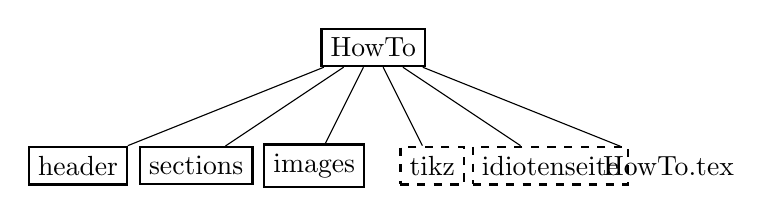
\begin{tikzpicture}
  \tikzstyle{folder}=[draw=black, thick]
  \tikzstyle{optional}=[dashed, folder]
  \node[folder] {HowTo}
    child {node[folder] {header}}
    child {node[folder] {sections}}
    child {node[folder] {images}}
    child {node[optional] {tikz}}
    child {node[optional] {idiotenseite}}
    child {node {HowTo.tex}};
\end{tikzpicture}
\end{lstlisting}


\subsubsection{Aufzählungen}
\url{http://www.ctan.org/pkg/enumitem}

\subsubsection{Bilder}
Zum Bilder einfügen: \url{http://www.ctan.org/tex-archive/macros/latex/required/graphics/} \\
Bilder in Tabellen: \url{http://www.ctan.org/pkg/adjustbox}

\subsubsection{Grafiken (TIKZ)}
\url{http://www.ctan.org/pkg/pgf}

\subsubsection{mehrere Spalten}
\url{http://www.ctan.org/pkg/multicol}


\subsubsection{Formeln}
\paragraph{Inline Formeln}
sind sehr praktisch wenn es nur darum geht etwas kurzes zu beschreiben oder einen Teil
einer anderen Formel zu erläutern. Zum Beispiel kann der Satz von Phytagoras so aussehen: $c^2 = a^2 + b^2$. Er kann jedoch auch
umgeformt werden und sieht dann so aus: $c=\sqrt{a^2 + b^2}$

\paragraph{Sonstige Formeln}
können mit den verschiedensten Umgebungen dargestellt werden. Am besten einfach in die Anleitungen der beiden Mathe-Packages
\href{http://www.ctan.org/pkg/amsmath}{amsmath}\footnote{\url{http://www.ctan.org/pkg/amsmath}} und 
\href{http://www.ctan.org/pkg/mathtools}{mathtools}\footnote{\url{http://www.ctan.org/pkg/mathtools}} schauen!
Einfache Formeln welche keine spezielle Umgebung benötigen sollten mit \verb+\[...\]+ geschrieben und nicht mit
\verb+$$...$$+. Die Form mit den Dollarzeichen hat zum Teil nicht erwünschte Nebeneffekte.
Folgendes Dokument ist nebst den Package-Dokumentationen auch lesenswert: 
\href{http://www.ctan.org/pkg/voss-mathmode}{Mathmode}\footnote{\url{http://www.ctan.org/pkg/voss-mathmode}}

\subsubsection{Tabellen}
\url{http://www.ctan.org/pkg/tabularx}
